\documentclass{article}
%
%
\makeatletter
\@ifundefined{lhs2tex.lhs2tex.sty.read}%
  {\@namedef{lhs2tex.lhs2tex.sty.read}{}%
   \newcommand\SkipToFmtEnd{}%
   \newcommand\EndFmtInput{}%
   \long\def\SkipToFmtEnd#1\EndFmtInput{}%
  }\SkipToFmtEnd

\newcommand\ReadOnlyOnce[1]{\@ifundefined{#1}{\@namedef{#1}{}}\SkipToFmtEnd}
\usepackage{amstext}
\usepackage{amssymb}
\usepackage{stmaryrd}
\DeclareFontFamily{OT1}{cmtex}{}
\DeclareFontShape{OT1}{cmtex}{m}{n}
  {<5><6><7><8>cmtex8
   <9>cmtex9
   <10><10.95><12><14.4><17.28><20.74><24.88>cmtex10}{}
\DeclareFontShape{OT1}{cmtex}{m}{it}
  {<-> ssub * cmtt/m/it}{}
\newcommand{\texfamily}{\fontfamily{cmtex}\selectfont}
\DeclareFontShape{OT1}{cmtt}{bx}{n}
  {<5><6><7><8>cmtt8
   <9>cmbtt9
   <10><10.95><12><14.4><17.28><20.74><24.88>cmbtt10}{}
\DeclareFontShape{OT1}{cmtex}{bx}{n}
  {<-> ssub * cmtt/bx/n}{}
\newcommand{\tex}[1]{\text{\texfamily#1}}	% NEU

\newcommand{\Sp}{\hskip.33334em\relax}
\newcommand{\NB}{\textbf{NB}}
\newcommand{\Todo}[1]{$\langle$\textbf{To do:}~#1$\rangle$}

\EndFmtInput
\makeatother
%
\usepackage{pgf}
\usepackage{tikz}
\usepackage[utf8]{inputenc}
\usetikzlibrary{arrows,automata}
\usetikzlibrary{positioning}
\tikzset{
    state/.style={
           rectangle,
           rounded corners,
           draw=black, very thick,
           minimum height=4em,
           minimum width=4em,
           fill=blue!10,
           inner sep=2pt,
           node distance=2cm,
           text centered,
           },
}
\author{Martin Drautzburg}

\title{The State Mondad slowly dissected}

\begin{document} \maketitle \tableofcontents 

\section{The type}
The type we are dealing with is the following:

\begin{tabbing}\texfamily
{\bfseries newtype}~{\itshape State}~s~a~=~{\itshape State}~\char123 ~runState~::~s~\char'31~(a,~s)~\char125 
\end{tabbing}

\subsection{Record syntax}

To get a feeling for what this \text{\texfamily {\itshape State}} type means, we will construct
such a type ourselves. First we need to understand the record syntax used
here.

Record syntax allows to define a tuple together with access functions
to retrieve specific components of the tuple. To understand the
motivation behind it, we will first try without record syntax.

\subsubsection{Tuples}
Consider a Pair of \text{\texfamily {\itshape Int}} and \text{\texfamily {\itshape String}}, where want to refer to the
first component as \text{\texfamily foo} and to the second component as \text{\texfamily bar}. With
such a type we can write access functions which retrieve either the
first or second component and which have a name which reflects the
name of the component.

\begin{tabbing}\texfamily
{\bfseries type}~{\itshape PairTuple}~=~({\itshape Int},~{\itshape String})\\
\texfamily fooTuple~(foo,\char95 )~=~foo\\
\texfamily barTuple~(\char95 ,bar)~=~bar
\end{tabbing}

If we want to modify one of the components, we need additional
functions like

\begin{tabbing}\texfamily
modFooTuple::{\itshape Int}\char'31{\itshape PairTuple}\char'31{\itshape PairTuple}\\
\texfamily modFooTuple~foo~(\char95 ,~bar)~=~(foo,~bar)\\
\texfamily \\
\texfamily modBarTuple::{\itshape String}\char'31{\itshape PairTuple}\char'31{\itshape PairTuple}\\
\texfamily modBarTuple~bar~(foo,\char95 )~=~(foo,~bar)
\end{tabbing}


As an exercise let's create a Pair and then modify each of the
components and retrieve the bar compnent

\begin{tabbing}\texfamily
ex1~=~barTuple~\$~(modBarTuple~\char34 changed\char34 )~\$~(modFooTuple~2)~\$~(1,\char34 init\char34 )
\end{tabbing}

\begin{tabbing}\tt
~\char42{}Main\char62{}~ex1\\
\tt ~\char34{}changed\char34{}\\
\tt ~\char42{}Main\char62{}~
\end{tabbing}

\subsubsection{Records}

It seems unneccessary to define these four functions, because all the
system needs to know is the types and names of the components. This is
where record syntax comes in. We cannot get away with a simple \text{\texfamily {\bfseries type}}
synonym anymore, but must define a new type, e.g. using the \text{\texfamily {\bfseries data}}
keyword.

\begin{tabbing}\texfamily
{\bfseries data}~{\itshape PairRecord}~=~{\itshape PR}~\char123 foo::{\itshape Int},~bar::{\itshape String}\char125 ~{\bfseries deriving}~({\itshape Eq},{\itshape Show})
\end{tabbing}

This definition magically creates two functions \text{\texfamily foo} and \text{\texfamily bar} which
correspond to the \text{\texfamily fooTuple} and \text{\texfamily barTuple} functions we created
ourselves in the previous example.

\begin{tabbing}\tt
~\char42{}Main\char62{}~\char58{}t~foo\\
\tt ~foo~\char58{}\char58{}~PairRecord~\char45{}\char62{}~Int\\
\tt ~\char42{}Main\char62{}~\char58{}t~bar\\
\tt ~bar~\char58{}\char58{}~PairRecord~\char45{}\char62{}~String
\end{tabbing}

Using record syntax, we can create \text{\texfamily {\itshape PairRecord}}s ...

\begin{tabbing}\texfamily
pr1~=~{\itshape PR}~\char123 foo=1,~bar=\char34 init\char34 \char125 
\end{tabbing}

retrieve the components ...

\begin{tabbing}\tt
~\char42{}Main\char62{}~foo~pr1\\
\tt ~1\\
\tt ~\char42{}Main\char62{}~bar~pr1\\
\tt ~\char34{}init\char34{}
\end{tabbing}

and even update records

\begin{tabbing}\tt
~\char42{}Main\char62{}~pr1~\char123{}bar~\char61{}~\char34{}changed\char34{}\char125{}\\
\tt ~PR~\char123{}foo~\char61{}~1\char44{}~bar~\char61{}~\char34{}changed\char34{}\char125{}\\
\tt ~\char42{}Main\char62{}~
\end{tabbing}

where an \emph{update} is of course not a real update, but the
construction of a new PairRecord with one or more components changed.

\subsection{A type with a function}

The \text{\texfamily {\itshape State}} type however, does not consist of simple types like \text{\texfamily {\itshape Int}}
and \text{\texfamily {\itshape String}} but wraps around a function. To get a feeling of what
this does, let's again create such a Type ourselves.

\begin{tabbing}\texfamily
{\bfseries data}~{\itshape FuncRecord}~=~{\itshape FR}\char123 run~::~{\itshape Int}\char'31{\itshape Int}\char125 
\end{tabbing}

To create such a record we must pass a function into the data
constructor \text{\texfamily {\itshape FR}}. This function could be an already existing function, or
one which we create on-thy-fly, using a lambda expression. Let's try both:

\begin{tabbing}\texfamily
inc~x~=~x+1\\
\texfamily frInc~=~{\itshape FR}~inc\\
\texfamily frDouble~=~{\itshape FR}~~(\char'10x~\char'31~x*2)
\end{tabbing}

So what we can do with such things? We know we can retrieve the \text{\texfamily run}
component, which will give us a function. This function can then be
applied to an argument.

\begin{tabbing}\tt
~\char42{}Main\char62{}~\char40{}run~frInc\char41{}~5\\
\tt ~6\\
\tt ~\char42{}Main\char62{}~\char40{}run~frDouble\char41{}~5\\
\tt ~10
\end{tabbing}

\section{Monads}

A Monad can often be seen as a \emph{something of something else}. If
you have a \text{\texfamily {\itshape List}} of \text{\texfamily {\itshape Int}}s, then the \emph{something} is \text{\texfamily {\itshape List}} and
the \emph{something else} is \text{\texfamily {\itshape Int}}.

In type signatures you often see a thing like \text{\texfamily {\itshape M}\Sp a} (or \text{\texfamily m\Sp a}). Here
\text{\texfamily {\itshape M}} is the \emph{something} and \text{\texfamily a} is the \emph{something else}. The
\text{\texfamily {\itshape M}} is called a \emph{type constructor} as it creates a new type from
a base type \text{\texfamily a}. If there was a type constructor \text{\texfamily {\itshape List}}, then a List
of Ints would be written as \text{\texfamily {\itshape List}\Sp {\itshape Int}}.

As far as monadic operations are concerned, the \text{\texfamily {\itshape Int}} is of little
concern. The monadic operators like \text{\texfamily return} and \text{\texfamily >>=} \text{\texfamily (\char34 bind\char34 )}are
spefic to the \emph{type constructors} only.

This kind of abstraction is very common in Haskell. E.g. the \text{\texfamily reverse}
operation on Lists works on Lists of any types. It knows nothing about
the type of elements in the List. This is the way it should be: "A
function which inverses a list of bananas knows nothing about bananas"

However, Mondads are not about reversing, but about chaining. It is a
good idea to know the type of the bind operator \text{\texfamily >>=} by heart.

\begin{tabbing}\tt
~\char40{}\char62{}\char62{}\char61{}\char41{}~\char58{}\char58{}~Monad~m~\char61{}\char62{}~m~a~\char45{}\char62{}~\char40{}a~\char45{}\char62{}~m~b\char41{}~\char45{}\char62{}~m~b
\end{tabbing}

This just sais, that \text{\texfamily (>>=)} creates a new monadic value from an old
monadic value with the help of a function. It sais nothing about
\emph{how} this is done. There are in fact several options, but mostly
one of them is overwhelmingly more useful than the others.


%\path [draw, thick, ->] (f1) edge[out=0, in=-90, in distance=2cm] node[below]{a} (g.south) ;

\subsection{A first monad}

Let's try to roll our own monad from our \text{\texfamily {\itshape FuncRecord}} from above. We
must change a number of things. First a monad needs a type variable
(the \emph{of something else}). So instead of functions from Int to
Int, we use functions from Int to some type \text{\texfamily a}. Then we must rename a
number of things, to avoid name clashes with our \text{\texfamily {\itshape FuncRecord}}

\begin{tabbing}\texfamily
{\bfseries data}~{\itshape FuncRecordMonad}~a~=~{\itshape FRM}\char123 runm~::~{\itshape Int}\char'31a\char125 \\
\texfamily \\
\texfamily {\rmfamily-{}-  some examples:}\\
\texfamily frmInc~=~{\itshape FRM}~(\char'10x~\char'31~x+1)\\
\texfamily frmDouble~=~{\itshape FRM}~(\char'10x~\char'31~x*2)
\end{tabbing}

The experiments we did with the \text{\texfamily {\itshape FR}} type will work with \text{\texfamily {\itshape FRM}} just as
well, namely \text{\texfamily (runm\Sp frmInc)\Sp 5} and  \text{\texfamily (runm\Sp frmDouble)\Sp 5}

To make \text{\texfamily {\itshape FRM}} a monad, we must define the two function \text{\texfamily return} and
\text{\texfamily (>>=)}.  

\subsubsection{Return}

The \text{\texfamily return} function \text{\texfamily return\Sp ::\Sp {\itshape Monad}\Sp m\Sp =>\Sp a\Sp \char'31\Sp m\Sp a} takes some value
and constructs a Monad from it. In our case thus would be a function,
which returns a value of type \text{\texfamily a}. There aren't too many options,
because the only variable whose type is definitly an \text{\texfamily a} is the
argument to \text{\texfamily return}, whose actual type is not known. So our only
option is to create a function, which returns this value regardless of
its input, somthing like $return\, x = FRM (\lambda \_ \rightarrow x)$

\bigskip

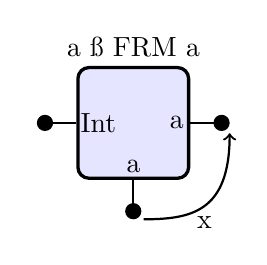
\begin{tikzpicture}
 \node[state, label=above:\text{\texfamily a\Sp \char'31\Sp {\itshape FRM}\Sp a}] (g) {};
 \draw [thick, -*] (g.east) ++(0,0.0)   node [xshift=-5pt]  {a} -- +(0.5,0)  node (gout) {};
 \draw [thick, -*] (g.west) ++(0,-0.0)  node [xshift=8pt]   {Int} -- +(-0.5,0) node (gain) {};
 \draw [thick, -*] (g.south) ++(0,-0.0) node [yshift=5pt]   {a} -- +(0,-0.5) node (gin2) {};

 \path [draw, thick, ->] (gin2) edge[out=0, in=-90, in distance=1cm] node[below]{\text{\texfamily x}} (gout) ;    
\end{tikzpicture}

\subsubsection{Bind}

Now we ask ourselved the question: if we have such a function, wrapped
in \text{\texfamily {\itshape FRM}} and a function which creates another such such function (the
\text{\texfamily a\Sp \char'31\Sp {\itshape M}\Sp b}), how can we construct a new \text{\texfamily {\itshape FRM}} in a way which makes some
sense?

\bigskip

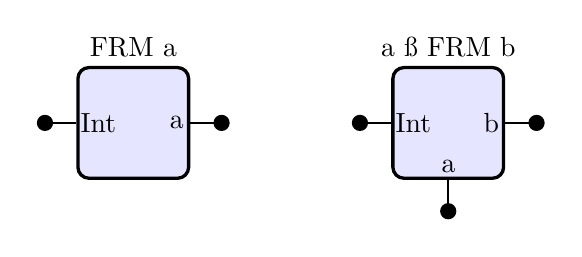
\begin{tikzpicture}
 \node[state, label=above:\text{\texfamily {\itshape FRM}\Sp a}] (f) {};
 \draw [thick, -*] (f.east) ++(0, 0.0) node [xshift=-5pt]  {a} -- +(0.5,0)  node (fout) {};
 \draw [thick, -*] (f.west) ++(0,-0.0) node [xshift=8pt]   {Int} -- +(-0.5,0) node (fin) {};

 \node[state, right of=f, xshift=2cm, label=above:\text{\texfamily a\Sp \char'31\Sp {\itshape FRM}\Sp b}] (g) {};
 \draw [thick, -*] (g.east) ++(0,0.0)   node [xshift=-5pt]  {b} -- +(0.5,0)  node (gout) {};
 \draw [thick, -*] (g.west) ++(0,-0.0)  node [xshift=8pt]   {Int} -- +(-0.5,0) node (gain) {};
 \draw [thick, -*] (g.south) ++(0,-0.0) node [yshift=5pt]   {a} -- +(0,-0.5) node (gin2) {};

\end{tikzpicture}



To implement \text{\texfamily (>>=)} we must combine these into a single
function. There aren't too many options. Remember that

\begin{tabbing}\tt
~\char40{}\char62{}\char62{}\char61{}\char41{}~\char58{}\char58{}~Monad~m~\char61{}\char62{}~m~a~\char45{}\char62{}~\char40{}a~\char45{}\char62{}~m~b\char41{}~\char45{}\char62{}~m~b
\end{tabbing}


The function \text{\texfamily \Sp a\Sp \char'31\Sp {\itshape M}\Sp b} expects an \text{\texfamily a}. We might feel tempted to pass
it some constant, but we do not really know its type. We only know it
is an "\text{\texfamily a}". So we cannot do this. The only way we can feed it an \text{\texfamily a}
is to take the return value from the first \text{\texfamily {\itshape FRM}}.

\bigskip

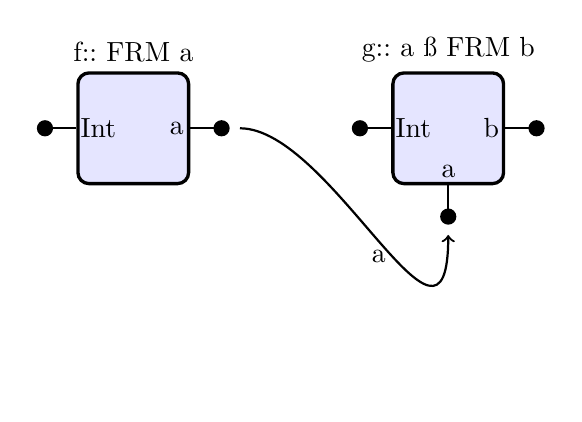
\begin{tikzpicture} 
\node[state, label=above:\text{\texfamily f::\Sp {\itshape FRM}\Sp a}] (f) {}; 
\draw [thick,-*] (f.east) ++(0, 0.0) node [xshift=-5pt] {a}   --+(0.5,0) node (fout){}; 
\draw [thick, -*] (f.west) ++(0,-0.0) node [xshift=8pt] {Int} --+(-0.5,0) node (fin) {};

 \node[state, right of=f, xshift=2cm, label=above:\text{\texfamily g::\Sp a\Sp \char'31\Sp {\itshape FRM}\Sp b}] (g) {};
 \draw [thick, -*] (g.east) ++(0,0.0)   node [xshift=-5pt]  {b} -- +(0.5,0)  node (gout) {};
 \draw [thick, -*] (g.west) ++(0,-0.0)  node [xshift=8pt]   {Int} -- +(-0.5,0) node (gain) {};
 \draw [thick, -*] (g.south) ++(0,-0.0) node [yshift=5pt]   {a} -- +(0,-0.5) node (gin2) {};

 \path [draw, thick, ->] (fout) edge[out=0, in=-90, in distance=2cm] node[below]{\text{\texfamily a}} (gin2) ;    
\end{tikzpicture}


We still have two \text{\texfamily {\itshape Int}} inputs, but the resulting function should have
only one. We could pass a constant \text{\texfamily {\itshape Int}} to the second
function. However the chosen value would be difficult to
justify. Instead we will pass the agrument to the first function also
to the second function.


\bigskip

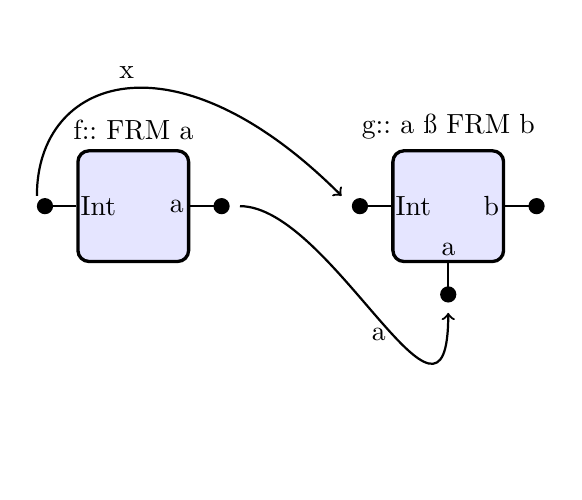
\begin{tikzpicture} 
\node[state, label=above:\text{\texfamily f::\Sp {\itshape FRM}\Sp a}] (f) {}; 
\draw [thick,-*] (f.east) ++(0, 0.0) node [xshift=-5pt] {a}   --+(0.5,0) node (fout){}; 
\draw [thick, -*] (f.west) ++(0,-0.0) node [xshift=8pt] {Int} --+(-0.5,0) node (fin) {};

 \node[state, right of=f, xshift=2cm, label=above:\text{\texfamily g::\Sp a\Sp \char'31\Sp {\itshape FRM}\Sp b}] (g) {};
 \draw [thick, -*] (g.east) ++(0,0.0)   node [xshift=-5pt]  {b}   -- +(0.5,0)  node (gout) {};
 \draw [thick, -*] (g.west) ++(0,-0.0)  node [xshift=8pt]   {Int} -- +(-0.5,0) node (gin) {};
 \draw [thick, -*] (g.south) ++(0,-0.0) node [yshift=5pt]   {a}   -- +(0,-0.5) node (gin2) {};

 \path [draw, thick, ->] (fout) edge[out=0, in=-90, in distance=2cm] node[below]{\text{\texfamily a}} (gin2) ;    
 \path [draw, thick, ->] (fin) edge[out=90, in=135, in distance=3cm] node[above]{\text{\texfamily x}} (gin) ;    
\end{tikzpicture}

The result indeed has the type \text{\texfamily {\itshape M}\Sp b}, i.e. \text{\texfamily {\itshape FRM}\Sp b}, a function from
\text{\texfamily {\itshape Int}} to \text{\texfamily b}. To write this in proper Haskell, we first apply \text{\texfamily f} to
\text{\texfamily x} by means of \text{\texfamily (runm\Sp f)\Sp x)}. This gives us some value of type
\text{\texfamily a}. We pass this value to \text{\texfamily g} which gives us another \text{\texfamily {\itshape FRM}\Sp b}. Finally
we apply this new function to the same \text{\texfamily x} and get a value of type
\text{\texfamily b}. So we have constructed a new function \text{\texfamily f2} from \text{\texfamily f} and \text{\texfamily g} and
the only thing left to do, is to wrap in inside \text{\texfamily {\itshape FRM}}.

\begin{tabbing}\texfamily
{\bfseries instance}~{\itshape Monad}~{\itshape FuncRecordMonad}~{\bfseries where}\\
\texfamily ~~~~~~~~return~x~=~{\itshape FRM}~(\char92 \char95 ~\char'31~~x)\\
\texfamily ~~~~~~~~f~>>=~g~=~{\itshape FRM}~f2\\
\texfamily ~~~~~~~~~~~~~~~~{\bfseries where}\\
\texfamily ~~~~~~~~~~~~~~~~~~~~f2~x~=~(runm~(g~((runm~f)~x)))~x
\end{tabbing}


\subsubsection{Doing}

We designed our monad with no specific purpose in mind. But let's
explore what it does anyways.

\text{\texfamily {\itshape Return}} alone would create a function which always returns the same
value To actually run this function we must unwrap it with \text{\texfamily runm}.

\begin{tabbing}\texfamily
f2~=~runm~frm\\
\texfamily ~~~~~~~~{\bfseries where}\\
\texfamily ~~~~~~~~~~~~frm~=~return~\char34 42\char34 
\end{tabbing}

\begin{tabbing}\tt
~\char42{}Main\char62{}~\char58{}t~f2\\
\tt ~f2~\char58{}\char58{}~Int~\char45{}\char62{}~\char91{}Char\char93{}\\
\tt ~\char42{}Main\char62{}~f2~1\\
\tt ~\char34{}42\char34{}\\
\tt ~\char42{}Main\char62{}~f2~2\\
\tt ~\char34{}42\char34{}
\end{tabbing}

Now let's try the chaining. We must invent that second function \text{\texfamily g\Sp ::\Sp a\Sp \char'31\Sp {\itshape FRM}\Sp b}, where the b-typed value inside \text{\texfamily {\itshape FRM}} is a function from
\text{\texfamily {\itshape Int}} to some type \text{\texfamily b}. 


\begin{tabbing}\texfamily
f3~=~runm~frm\\
\texfamily ~~~~~~~~{\bfseries where}\\
\texfamily ~~~~~~~~~~~~frm~=~return~\char34 42\char34 ~>>=~\char'10a~\char'31~{\itshape FRM}~(\char'10x~\char'31~(show~x)~++~a)~
\end{tabbing}

So this function returns its agument suffixed by the String \text{\texfamily 42}.


\begin{tabbing}\tt
~\char42{}Main\char62{}~f3~1\\
\tt ~\char34{}142\char34{}\\
\tt ~\char42{}Main\char62{}~f3~99\\
\tt ~\char34{}9942\char34{}
\end{tabbing}

Now, let's try to rewrite \text{\texfamily f3} using do-notation. First, let's try to
get rid of the value constructor \text{\texfamily {\itshape FRM}} by using \text{\texfamily return}. Furthermore
let's get rid of the lambda by making it an argument to \text{\texfamily f3}. Finally
let's not unwrap right away, using \text{\texfamily runm} but return a
\text{\texfamily {\itshape FuncRecordMonad}} and leave the unwapping to the caller.

\begin{tabbing}\texfamily
f3a~x~=~return~\char34 42\char34 ~>>=~\char'10a~\char'31~return~((show~x)~++~a)~\\
\texfamily \\
\texfamily {\rmfamily-{}-  This translates to do-notation}\\
\texfamily f3b~x~=~{\bfseries do}\\
\texfamily ~~~~a~\char'30~(return~\char34 42\char34 )~::~{\itshape FuncRecordMonad}~{\itshape String}\\
\texfamily ~~~~return~((show~x)~++~a)~
\end{tabbing}

The type of \text{\texfamily f3b} is now \text{\texfamily \Sp f3b\Sp ::\Sp {\itshape Show}\Sp a\Sp =>\Sp a\Sp \char'31\Sp {\itshape FuncRecordMonad}\Sp [{\itshape Char}]\Sp }. If we pass it one parameter,
we get \text{\texfamily \Sp f3b\Sp 99\Sp ::\Sp {\itshape Num}\Sp a\Sp =>\Sp {\itshape FuncRecordMonad}\Sp [{\itshape Char}]\Sp } from which we can extract the function
\text{\texfamily \Sp runm\Sp (f3a\Sp 99)\Sp ::\Sp {\itshape Num}\Sp a\Sp =>\Sp {\itshape Int}\Sp \char'31\Sp [{\itshape Char}]\Sp } and when we finally call this function we get:

\begin{tabbing}\tt
~\char42{}Main\char62{}~\char40{}runm~\char40{}f3b~99\char41{}\char41{}~666\\
\tt ~\char34{}9942\char34{}
\end{tabbing}

Note that the final argument 666 is actually ignored. The result only
depends on \text{\texfamily x=99}, the parameter we passed first to f3b. Let's try to
construct a more intelligent \text{\texfamily {\itshape FuncRecordMonad}}, one which transforms
an existing \text{\texfamily {\itshape FuncRecordMonad}}.

\begin{tabbing}\texfamily
f4~frm~=~{\bfseries do}\\
\texfamily ~~~~a~\char'30~frm~::~{\itshape FuncRecordMonad}~{\itshape String}\\
\texfamily ~~~~b~\char'30~{\itshape FRM}~\$~\char'10x~\char'31~(x~+~length~a)\\
\texfamily ~~~~return~b
\end{tabbing}


\text{\texfamily f4} takes some wrapped \text{\texfamily {\itshape Int}\Sp \char'31\Sp {\itshape String}} function and returns a
function, which adds the length of the String to its \text{\texfamily {\itshape Int}} parameter.


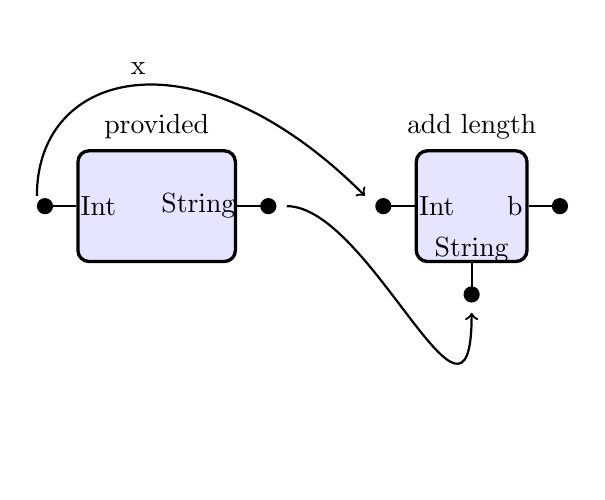
\begin{tikzpicture} 
\node[state, minimum width=2cm, label=above:\text{\texfamily provided}] (f) {}; 
\draw [thick,-*] (f.east) ++(0, 0.0) node [xshift=-14pt] {String}   --+(0.5,0) node (fout){}; 
\draw [thick, -*] (f.west) ++(0,-0.0) node [xshift=8pt] {Int} --+(-0.5,0) node (fin) {};

 \node[state, right of=f, xshift=2cm, label=above:\text{\texfamily add\Sp length}] (g) {};
 \draw [thick, -*] (g.east) ++(0,0.0)   node [xshift=-5pt]  {b}   -- +(0.5,0)  node (gout) {};
 \draw [thick, -*] (g.west) ++(0,-0.0)  node [xshift=8pt]   {Int} -- +(-0.5,0) node (gin) {};
 \draw [thick, -*] (g.south) ++(0,-0.0) node [yshift=5pt]   {String}   -- +(0,-0.5) node (gin2) {};

 \path [draw, thick, ->] (fout) edge[out=0, in=-90, in distance=2cm] node[below]{} (gin2) ;    
 \path [draw, thick, ->] (fin) edge[out=90, in=135, in distance=3cm] node[above]{\text{\texfamily x}} (gin) ;    
\end{tikzpicture}

\begin{tabbing}\tt
~\char42{}Main\char62{}~~\char40{}runm~\char36{}~f4~\char40{}FRM~\char36{}~\char92{}x~\char45{}\char62{}~show~x\char41{}\char41{}~120\\
\tt ~123\\
\tt ~\char42{}Main\char62{}~~\char40{}runm~\char36{}~f4~\char40{}FRM~\char36{}~\char92{}x~\char45{}\char62{}~take~x~\char34{}lkjlkjl\char34{}\char41{}\char41{}~10\\
\tt ~17
\end{tabbing}

\end{document}
